\subsection{Qubit}
\label{Subsec: Qubit}

\paragraph{}One qubit is a subspace with two dimensions, that means we can map a qubit to $\mathbf{C}^2$ . We can choose a basis in order to span this vector space, we will choose the standard computational basis that will be associated to bits:
\begin{equation}
\label{Eq: Computational Basis}
\ket{0} =  
\begin{pmatrix} 
1 \\
0 \\
\end{pmatrix}
\
and
\
\ket{1} =  
\begin{pmatrix} 
0 \\
1 \\
\end{pmatrix}
\end{equation}

The general state of a qubit is a superposition of those states:

\begin{equation}
\label{Eq: Superposition of qubit}
\ket{\psi} = \alpha \ket{0} + \beta \ket{1}
\end{equation}

This state can be parameterized by two parameters and construct what we call a "Bloch Sphere":
\begin{equation}
\label{Eq: Bloch Sphere}
\ket{\psi} = cos\left(\frac{\theta}{2} \right) \ket{0} + e^{i\phi}sin\left(\frac{\theta}{2} \right) \ket{1}
\end{equation}

\begin{figure}[H]
\centering
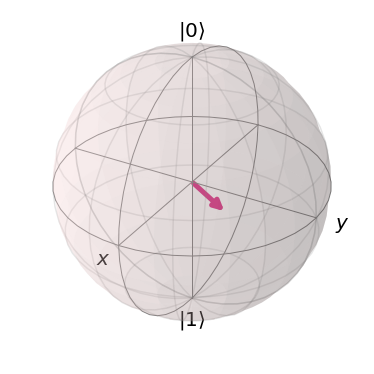
\includegraphics[width=0.3\textwidth]{Figures/bloch.png}
\caption{Graphical representation of the Bloch sphere.}
\end{figure}